%!TEX root = ../prelims_main.tex
% \documentclass[../prelims_main.tex]{subfiles}

% \begin{document}

\section{Introduction}
\begin{multicols}{2}

\subsection{Outline}

\begin{itemize}
	\item Language Games
	\begin{itemize}
		\item Category structure of phonemes
		\item family resemlances in cognitive lit - why is phonetic identification a family resemblance strucutre?
		\item general statement of geometry of perceptual spaces
		\item family resemblances that differ in many senses really are defined by contrast between them -- which sense lets me distinguish the objects in question? put another way, selecting or rotating axes depending on short-term acoustic statistics.
		\item update to idea of perceptual geometry to include contextual dependence and reweighting
		\item Primary object is to learn the axes -- rather than learning some prebuilt structure that `exists in the world', brain has to figure out what parts of the world are informative, which is necessarily in context
	\end{itemize}

	\item Learning to play
	\begin{itemize}
		\item Infant speech learning, statistical regularity, perceptual warping
		\item general statement about the normalization of redundancy and adaptation to statistical regularity as a fundamental part of the auditory system (or maybe a brief allusion to it and discuss in more detail in neurophys section)
		\item But perceptual systems don't find `totally optimal' solutions as might be predicted from simpler experiments... 
		\item Representativeness means that there will be contributions from all the feature axes, even when they're irrelevant in the particular context.
	\end{itemize}

	\item Neurophys
	\begin{itemize}
		\item 
	\end{itemize}

\end{itemize}


\subsection{Phonemes are Language Games}

\begin{leftbar}

"Consider for example the proceedings that we call "games". [...] For if you look at them you will not see something that is common to all, but similarities, relationships, and a whole series of them at that. [...] Are they all 'amusing'? Compare chess with noughts and crosses. Or is there always winning and losing, or competition between players? Think of patience. [...] Look at the parts played by skill and luck; and at the difference between skill in chess and skill in tennis. 

And the result of this examination is: we see a complicated network
of similarities overlapping and criss-crossing: sometimes overall similarities, sometimes similarities of detail. [...] And we extend our concept as in spinning a thread we twist fibre on fibre. And the strength of the thread does not reside in the fact that some one fibre runs through its whole length, but in the overlapping of many fibres."

\textit{-Wittgenstein, Philosophical Investigations: 66-67\cite{wittgensteinPhilosophicalInvestigations1968}}

\end{leftbar}

Cognitive reality is characterized by its discreteness: rather than a continuous undifferentiated gradient wash of sensation and cognition, we experience objects, concepts, and categories. Speech is a continuous, high-dimensional, high-variability acoustic signal, yet it is perceived as a small number of relatively-discrete phonemes\cite{holtSpeechPerceptionCategorization2010a}. The acoustic structure of phonemes is a sort of "Family Resemblance"\cite{wittgensteinPhilosophicalInvestigations1968} --- the truly extravagant variability of speech has thus far defied any simple, definite acoustic parameterization of its phonemes. Instead, individual utterances within a phonetic category vary along high numbers of feature-dimensions, none of which are necessary nor sufficient for a listener to identify it\cite{Lisker1977}.

\draft{There are different types of category structure, and what typifies family resemblance structures is 1) multiply defined - category membership is assesed across many imperfect `features' none of which is necessary nor sufficient, 2) prototypicality - some instances are better `examples' of a category than others, category membership is not binary, 3) context dependent - which feature is important depends on the features present in the instance and the context in which it is being compared. \cite{roschFamilyResemblancesStudies1975}}

\subsection{A Very Simple Model...}

To begin perhaps purposely naively, we will formulate a geometric conception of perceptual categories:

Suppose that some sensory stimulus $\mathbf{s}$ was composed of some set of physical attributes $a_i$ in the $d$-dimensional "stimulus space" $\mathbf{S}$ capable of fully representing all stimuli for a given sensory modality (as opposed to a particular set of eg. parameterized stimuli)

\begin{equation}
\label{eqn:s}
\mathbf{s} = \{a_0, a_i, \dots a_d\ : a \in \mathbf{S}\}
\end{equation}

For example, a digital sound is fully defined by the amplitudes of the waveform at each of its samples, or an image is defined as the wavelength and intensity of light at each pixel.  Since $a_i$ are arbitrary, $\mathbf{S}$ can represent a set of static attributes, or a set of attributes through time.

The sensory stimulus $\mathbf{s}$ is processed into some percept $\mathbf{p}$ composed of perceptual attributes $b_i$ in the $e$-dimensional "perceptual space" $\mathbf{P}$

\begin{equation}
\label{eqn:p}
\mathbf{p} = \{b_0, b_i, \dots b_e\ : b \in \mathbf{P}\}
\end{equation}

such that some perceptual computation $M$ maps $\mathbf{S}$ to $\mathbf{P}$

\begin{equation}
\label{eqn:map}
M = f: \mathbf{S} \to \mathbf{P}
\end{equation} 

\begin{equation}
\label{eqn:pfroms}
\mathbf{p} = M(\mathbf{s})
\end{equation}

from which the objective of the observer is to infer the category $c_s$ given $\mathbf{s}$ 

\begin{equation}
\label{eqn:infer}
c_s = max( \{ p(c_i | \mathbf{p}) : c_i \in \mathbf{C} \})
\end{equation}

The form of the sensory-perceptual mapping $M$, the perceptual space $\mathbf{P}$ it constructs, and the inference of category identity $c_s$ it supports serve as a loom for a few threads of the speech perception problem scattered across a few disciplines and vocabularies.

\subsection{...and its history}

\idea{Make sure to refer back to the 3 properties of family resemblance categories and use that to structure this section!!!}

A prominent strain of phonetics research in the US, largely associated with the Haskins Labs (\cite{schertzPhoneticCueWeighting2020} and see \cite[p.~51]{ohalaGuideHistoryPhonetic1999}), has characterized the speech perception problem as resolving a set of acoustic "cues" into phonetic identity:

\begin{leftbar}
"Liberman, Cooper, and Pierre Delattre began to study the acoustic speech signal, to determine how it represents the consonants and vowels of spoken words, and to discover the acoustic structure (the `cues') essential for their identification by listeners. [\dots] By selectively including and eliminating elements of acoustic structure,l Liberman and his colleagues could determine what bits of structure provided information for the different phonetic properties of spoken words."

-Carol Fowler \& Katherine S. Harris in \cite[p.~51]{ohalaGuideHistoryPhonetic1999}
\end{leftbar}

The "cue discovery" paradigm of phonetics research posits that, for the auditory component of phonetic perception, the elements in $\mathbf{P}$ are linear combinations of the features in $\mathbf{S}$ whose manipulation can influence the identity of the perceived phoneme. These features represent familiar phonetic parameterizations like voice onset times or formant frequency ratios. The mapping $M$ that constructs $\mathbf{p}$ is taken to be a fixed, innate feature of the auditory system: "this version of the auditory theory takes the perceived boundary between one phonetic category and another to correspond to a naturally-occurring discontinuity in perception of the relevant acoustic continuum." \cite{Liberman1985a}. 

The conclusion of cue-based research is summarized neatly by Philip, Robert E. Remez, and Jennifer Pardo with respect to their sinewave synthesis experiments: "Question: Which acoustic elements are essential for the perception of speech? Answer: None\cite{HaskinsLaboratories2020}." The failure to find a simple parameterization of phonetic categories as acoustic cues motivated an abandonment of an acoustic account of phonetic perception entirely in favor of a motor theory of perception that positied a special, evolved "speech module" that linked the wily acoustics of speech sounds to the action of the articulatory system:

\begin{leftbar}
"For if phonetic categories were acoustic patterns, and if, accordingly, phonetic perception were properly auditory, one should be able to describe quite straightforwardly the acoustic basis for the phonetic category and its associated percept. According to the motor theory, by contrast, one would expect the acoustic signal to serve only as a source of information about the gestures; hence the gestures would properly define the category"
\cite{Liberman1985a}
\end{leftbar}

Purely motor theories of speech have been diversely problematized, not least of all by the many demonstrations that animals that conspicuously lack a human articulatory system are capable of phonetic categorization\cite{Carbonell2014,Lotto1997,Kluender2000}. The acoustic problem of speech perception was simply too difficult to be solved by an evolutionarily plausible auditory system -- how could the family resemblance structure of phonetic categories be learned without some explicit, innate knowledge of the acoustic consequences of articulation?\cite{Bailey1980} 

Research on infant acquisition of speech sounds has since demonstrated the profound plasticity of the auditory system and its ability to learn the complex statistical dependencies between the acoustic attributes of speech\cite{kuhlNewViewLanguage2000}. A family of models based primarily on the work of Patricia Kuhl and colleagues describe the stimulus space $\mathbf{S}$ as acoustic features based on the "basic cuts" of sensitivity in the auditory system\cite{kuhlEarlyLanguageAcquisition2004}. Infants exploit the statistical regularity and patterns of feature co-uccurance to learn some mapping $M$ that constructs a "warped" perceptual space $\mathbf{P}$ that clusters features in $\mathbf{S}$ into acoustic "prototypes."\cite{kuhlNewViewLanguage2000} 

Phonetic category identity then consists of some density in $\mathbf{P}$, the center of which is the "ideal" phonetic exemplar most likely to be identified with a particular categoery, and proceeding from this center point one transitions from off-target imperfect examplars to overlapping densities of other phonetic categories. Extensions to the model make this formulation explicit, like Kronrod, Coppess, and Feldman's\cite{Kronrod2016a} bayesian model that offers a unified explanation of the strong categorical perception of stop consonants and the weaker categorical perception of vowels. Their model describes phonetic identification as an inference problem that depends on both the acoustic properties of a stimulus and prior knowledge of phonetic categories, defined as some mean and variance in an arbitrary perceptual space. 

\draft{In this model, the difficulty of the acoustic problem of speech perception carefully described by cue-centric phonetic research is resolved by suggesting the auditory system relies on sharp internal representations of category identity for phonemes that have a large degree of uninformative variaance, like stop consonants.} 

\draft{The degree of arbitrariness is problematic for the model, however. The proposition that there is some stimulus space $\mathbf{P}$ that supports linearly-separable phonetic categories is emphatically counterevidenced by the 70 years of cue-based research that has attempted to find one (cite violations of gestalt principles from \cite{remezPerceptualOrganizationSpeech1994} and \cite{Lisker1977}). These prototype models, without weighting for the informativeness of a particular dimension in context (as opposed to some global weight) would be vulnerable to misidentifying speech when the most dominant cue was made redundant, when in fact human listeners will adapt to using a more informative cue. In fact a lot of the research relies on carefully parameterized speech, so if they considered the cases where those cues failed then such a single-density-based prototype model. Having nonlinear blobby parameterizations of prototypes doesn't really solve the problem either, as you would then just require an additional downstream `readout' layer that could compute the conditions where a particular dimension }


\draft{Their future directions says that identifying and learning the dimensions is of critical importance, we can extend our model by continuing Kronrod's emphasis on the information contained in each perceptual dimension and allow it to vary by context...}

\subsection{An extension to our model...}

Instead of a static perceptual space $\mathbf{P}$ where a given stimulus $\mathbf{s}$ is mapped to a single percept $\mathbf{p}$ (ie. $M$ is injective), we can extend our very simple model by introducing some notion of reweighting perceptual dimensions. Rather than inferring category directly from $\mathbf{P}$ as in eq. \ref{eqn:infer}, the features $b_e \in \mathbf{P}$ are reweighted by some weight vector $\mathbf{w}$ computed as some function $W$ of the representation $\mathbf{p} = M(\mathbf{s})$ and some prior knowledge of the category structure of $\mathbf{C}$

\begin{equation}
\label{eqn:w}
\mathbf{w} = W(\mathbf{p}, \mathbf{C})
\end{equation}

\begin{equation}
\label{eqn:infer_2}
c_s = max\big( \big\{ p(c_i | \mathbf{p} \cdot \mathbf{w}) : c_i \in \mathbf{C} \big\}\big)
\end{equation}

Recall that since the features $a \in \mathbf{S}$ are arbitrary, they can include time-varying features, so the weighting function $W$ can, for example, incorporate contextual effects from the recent perceptual past. Category inference being dependent on $W$ has equivalent interpretations in the parlance of artificial neural networks and geometry: as a self-attention mechanism (eg. \cite{vaswaniAttentionAllYou2017}) giving higher weight to more informative features, or as "collapsing" or "expanding" un/informative dimensions. 

\subsection{And its implications...}

The notion of different perceptual features having different weights or importance depending on the acoustic context and the category structure of the phonemes for a particular language is of course far from new. 

A parallel line of thought to the generative models that posit phonetic identity as some positive description of cues or perceptual features are discriminative models that focuses on the features that can be used to tell phonemes apart. A prominent family of discriminative models in phonetics are those that describe a hierarchy of contrastive features\cite{Dresher2008,clementsFeatureOrganization2006,halleFeatureSpreadingRepresentation2000}. Though they are diverse in their details, in these models $M$ is again typically some fixed feature of the auditory system, and the perceptual space $\mathbf{P}$ that it constructs is some set of high-level descriptions like voicing, frication, or articulator configuration. Typically these features are binary (eg. +/- voiced), rather than continuous.

\begin{figure}[H]
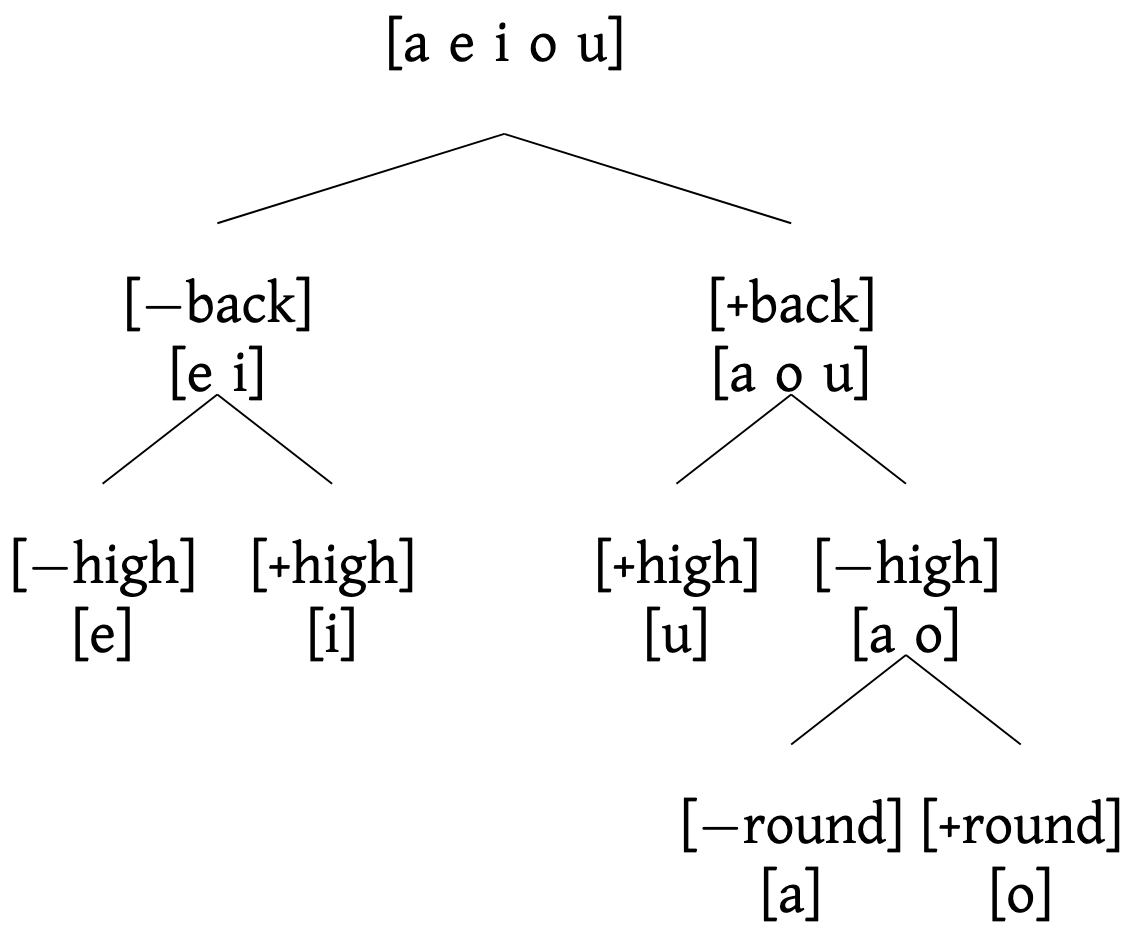
\includegraphics[width=\columnwidth]{russian_vowel_hierarchy.png}
\caption{Contrastive hierarchy for Russian Vowels, reproduced from \cite{iosadVowelReductionRussian2012} without permission}
\label{fig:hierarchy}
\end{figure}

As an example, consider the proposed contrastive feature hierarchy for russian vowels from \cite{iosadVowelReductionRussian2012} (Figure \ref{fig:hierarchy}). Vowel identification is dominated by the primary contrast of +/- back, and successive constrastive features eliminate candidate phonemes until the true phoneme is identified. $W$'s dependence on $\mathbf{C}$ is exemplified (\draft{fix passive voice..}) by its treatment of "round": -back vowels [e i] are fully determined by +/- high, so for a percept $\mathbf{p}$ with -back, the weight of "round" should be 0. Put another way, the importance of a given feature is dependent on the phonemes that are left ambiguous without it. Any given feature's importance depends on both the set of available features and the set of available categories. 

\draft{features like +rhotic though don't correspond to anything in the input space tho\cite{lindauStory1980}}

\todo{expand here on how parameterized stimuli with a single contrast aren't really modeling the problem: like shouldn't it matter how bad the speech sounds sound for claims about natural speech perception? the real question is, during perception, how are the different perceptual axes normalized/selected/weighted; during learning, how does the auditory system learn the space of features? When there is only one feature present the auditory system is performing a qualitatively different task. The use of parameterized stimuli is itself a strong assumption on the nature of the problem that the auditory system is solving. Even parameterizing a family resemblance is so because you assume the weight and salience of different cues. Additionally since there is some "basic cuts" argument to be made about the auditory system and the types of cues that it selects, you're unlikely to hit those if you just use some arbitrary array of stimuli: speech sounds come pre-optimized for mammalian auditory systems (though obvs mice aren't people) a la adaptive dispersion }

\draft{"I should emphasize, nevertheless, that there is a great deal of evidence that practice, even large amounts of it, does not produce efficient perception of acoustic alphabets. This is clear, not only in the example of the Morse code, but even more convincingly, perhaps, in the repeatedly unsuccessful attempts to find nonspeech sounds that will work well as part of a reading machine for the bling. Many sound alphabets have been given a thorough trial, but none has proved adequate. It must surely give us pause to know that, while sounds are the universal carriers of language, only one set of sounds --- those of speech --- serves well."\cite{libermanCharacteristicsPerceptionSpeech1970} Their conclusions are wrong -- that this means that speech is special and has its own processing modality -- but the observation does indeed point to the joint optimization of a phonetic space over an auditory space as being constitutive of language, and a potent reason to use speech sounds for category learning.}


The notion of the informativeness of different featural dimensions has been given its \draft{fullest} treatment in Keith Kluender and Christian Stilp's application of information theory to phonetic perception\cite{kluenderLongstandingProblemsSpeech2019a,kluenderPerceptionVowelSounds2013,stilpEfficientCodingStatistically2012,stilpRapidEfficientCoding2010}. They summarize their argument, elegantly as always:

\begin{leftbar}
"If one's problem is finding the right fencing to corral a unicorn, then there is really no problem at all. Instead the problem is dissolved upon discovery that unicorns do not exist.

Here, we ask the reader to consider the possibility that there are no objects of perception [...]. Like unicorns, they do not exist at all. Instead, there are \textit{objectives} for perception. [...] Perceptual success does not require recovery or representations of the world per se." \cite{kluenderLongstandingProblemsSpeech2019a}
\end{leftbar}

They argue that the central operation of sensory systems is to adapt to regularity at multiple scales in order to efficiently extract meaningful information from their environment. Rather than a faithful representation of articulatory maneuvers (as in motor theory) or a warped, but still bijective relationship between the acoustic space and perceptual space (as in perceptual warping), they argue that sensory systems discard information that is predictable based on (multiscale) context, and instead represent just the unpredictable, "information-bearing" in an appropriately Shannonistic sense, dimensions. 

Though theoretically all configurations of frequencies and amplitudes are possible, naturally produced sounds are strongly constrained by the physics of their production -- much of the variation in natural sounds is predictable. Rather than representing the fullness of acoustic variation, the auditory system adapts to redundancies and regularities in sounds to preferentially represent only the unpredictable, informative variation in an "efficient code" \cite{smithEfficientAuditoryCoding2006a,Geffen2011}. In the case of phonetic perception, where the objective of the listener is to identify the phoneme intended by the speaker rather than perceiving a sound qua sound, the listener attempts to learn auditory features that are maximally informative of phonetic identity\cite{kiefteAbsorptionReliableSpectral2008,liuOptimalFeaturesAuditory2019,kluenderLongstandingProblemsSpeech2019a,kluenderPerceptionVowelSounds2013}.

This information-theoretic account provides a mechanism for learning the dimensions of $\mathbf{P}$ and the form of $W$. Rather than some a priori, fixed inventory of articulatory/acoustic cues, a listener should learn some set of perceptual features that support the identification of phonemes given the phonemic inventory of their language and the acoustic variability (eg. accent, environment, timbre, etc.) that they are exposed to. Individual listeners do indeed use different combinations of cues with different weights\cite{iversonInfluencesPhoneticIdentification1996} which are stable over time\cite{souzaReliabilityRepeatabilitySpeech2018}. Rather than learning some category center and spread over some pre-existing perceptual feature space, the task of the listener is to learn the feature space itself. 

The difference between learning $\mathbf{P}$ and the operation of $W$ is a matter of timescale: over short timescales, $W$ reweights the features in $\mathbf{P}$ depending on those features that are contextually informative of phonetic identity. While the observation that individual cues are informative, uninformative, and anti-informative depending on the context of surrounding phonemes is a central feature of argument for a motor theory\cite{Bailey1980}, an information-theoretic view interprets this problem as a reweighting of individual features: /s/ differs from /f/ along different featural axes than /s/ differs from /k/, so /s/ shouldn't necessarily rely on the same inventory of acoustic features in all contexts. Contextual effects on phonetic categorization are of course well known (see \cite{holtSpeechPerceptionCategorization2010a}). Where perceptual warping accounts cannot explain results where some or all of the typical acoustic features are replaced, like sine-wave speech\cite{remezSpeechPerceptionTraditional1981}, noise-vocoded speech\cite{davisLexicalInformationDrives2005}, or joint spectrotemporal degradation\cite{elliottModulationTransferFunction2009a}; an information-theoretic view argues that listeners will adapt to use any cues that are still present (as in \cite{kiefteAbsorptionReliableSpectral2008}). 

The auditory system does \textit{not} seem to operate in an entirely information-maximizing way when identifying phonemes, however. Consider a category structure like that used by Couchman, Coutinho, and Smith (2010, \cite{couchmanRulesResemblanceTheir2010}) depicted in figure \ref{fig:rule_based}. Each stimulus is composed of four binary features (columns), and stimulus identity is defined by the first feature (0 = category A, 1 = category B). The remaining three features are "epiphenomenal," but stimuli in category B have a greater sum than those in category A. A perfect, information-maximizing observer would learn to only attend to the first dimension, but in speech and many other perceptual categories observers use many, even uninformative dimensions\cite{couchmanRulesResemblanceTheir2010,roschFamilyResemblancesStudies1975} (but see \cite{leaUseMultipleDimensions2008}). Non-speech sounds that are strictly uninformative of phonetic identity like pure tones and sweeps can nevertheless strongly influence the perceived phoneme\cite{holtNeighboringSpectralContent2000,holtMeanMattersEffects2006}, even when the sounds are not immediately adjacent\cite{holtTemporallyNonadjacentNonlinguistic2005}. Such an influence of many, imperfect stimulus dimensions on perception is our signpost to indicate we've arrived back in the bewildering little shire of category structures with family resemblance.

The differing (often implicit) assumptions about the \sarcasm{very complicated model™} characterize the major historical disputes in categorical phonetic perception, but also \draft{<suggest the kinds of experiments that might resolve them>.}

\todo{expand on each of these: a)} Arguably, the careful work of cue theorists led them to motor theories of perception because of a characterization of $M$ as fixed that made the non-invariant acoustic structure of phonetic categories impossible for the auditory system to compute. \draft{but their work was extremely valuable because it explicated the nonlinear nature of acoustic cues and the family resemblance structure of acoustic properties.} \todo{b)} Work in animal models and infant speech perception demonstrated that phonetic categories were indeed learned \todo{(cite infants can acquire all phonemes)}, but the use of parametric stimuli led to overly-parsimonious models that don't capture the true scope of the problem. \todo{need experiments that satisfy the "real problem" (review previous sections and highlight each of the ways the family resemblance structure of phonemes indicates a particular experimental design parameter, but that we need to finish it by adding a neural layer... which we get to in the next section...)}

 \begin{figure}[H]
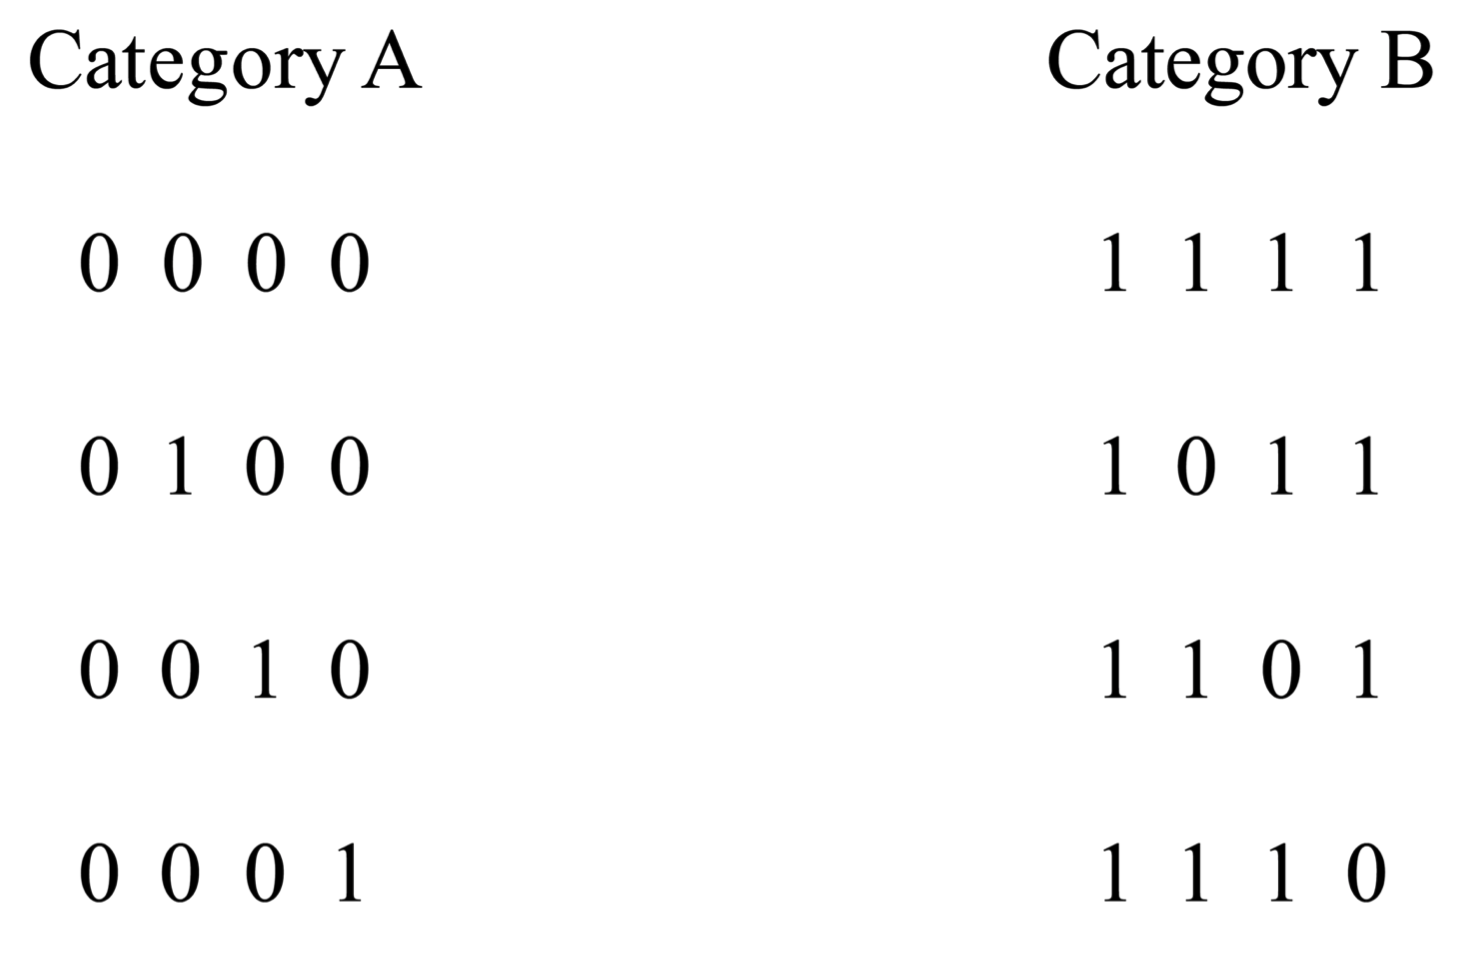
\includegraphics[width=\columnwidth]{rule_based_categorization.png}
\caption{Category structure reproduced from \cite{couchmanRulesResemblanceTheir2010} without permission. Each stimulus (row of four digits) is composed of four features (columns). Category identity is determined by the first feature (0 = A, 1 = B), but three other "irrelevant" features are present.}
\label{fig:rule_based}
\end{figure}




------------------

\draft{don't fuck up and forget to talk about these \cite{aravamudhanPerceptualContextEffects2008,holtMeanMattersEffects2006,holtTemporallyNonadjacentNonlinguistic2005}}

If $P$ is discrete, and the process of assigning category is feature comparison, we get tversky


Feature selection provides a plausible explanation also for the SWS experiments -- when all the traditional acoustic cues are absent, the auditory system is capable of adapting to the cues that are present even if they're totally unbelievable if they're based on purely on the expected covariance of the signal\cite{remezSpeechPerceptionTraditional1981} -- when told what speech to expect, it's easier to choose the axes to focus on -- there seems to be a dual process where a certain amount of contextual information needs to be present in order to cue the selection, but there's no reason that needs to be a fully distinct process.

Category membership is computed probabilistically from some configuration space $\phi$...



\textbf{Evidence supporting the family resemblance argument}
\begin{itemize}
	\item phonetic contrasts are multiply defined\cite{Lisker1977,Bailey1980}
	\item Cognitive categorization learning mostly operates as family resemblances that have incomplete/nonplatonic feature sets that unite them (\cite{roschFamilyResemblancesStudies1975}\cite{roschWittgensteinCategorizationResearch1987} \cite{couchmanRulesResemblanceTheir2010})
	\item tversky talked about this in terms of set theory and resemblance \cite{tverskyStudiesSimilarity1978} \cite{Tversky1970}
	\item People can switch discriminatory dimension depending on which is predictable vs. informative -- people use whatever cue is present and informative \cite{kiefteAbsorptionReliableSpectral2008} and it's relatively stable within a person \cite{souzaReliabilityRepeatabilitySpeech2018}
	\item animals use family resemblance of multiple features even when there is a single dimension that is perfectly informative of category membership \cite{leaUseMultipleDimensions2008, couchmanRulesResemblanceTheir2010}

\end{itemize}

\textbf{Different ways perceptual geometry gets talked about}
\begin{itemize}
	\item perceptual warping
	\item bayesian modeling of cues
	\item exploiting the statistical regularity to extract maximally informative dimensions
	\item contrast hierarchy <-> tversky's trees in features of similarity, tversky's objections can also be re-expressed as a crit of shitty geometry, rather than abandoning geometry, we need to estimate a geometry that does operate metrically (even if the dimensions operate categorically rather than continuously) (though he does consider weights here \cite{ritovDifferentialWeightingCommon1990})
\end{itemize}

\textbf{Crits of basic geometry case and relationship with existing ways of talking abt it in order to introduce the importance of `feature selection'}


Category representation theories are intimately related (and occasionally literally isometric to \cite{Edelman1998}) to theories of the measurement of similarity, which is dominated by geometric models\cite{Tversky1977}. nearly universally presuppose that categories exist in a feature space such that there exist some number of features that describe each instance of an object to be categorized.

The history of this question includes Shepard and Tversky's multidimensional scaling and its criticisms, and also extends through Shepherds' "second-order isomorphisms" (cite representation is representation of similarity)

Neuroscientists sorta blithely assume what the features of a stimulus are, from the seemingly harmless and physically based -- frequency, direction, angle, etc. -- to the absurd -- rsa et al. But these dimensions rarely behave like `real' perceptual dimensions \cite{krantzSimilarityRectanglesAnalysis1975a} -- the transformation is actually the critical part. 

assuming feature dimensions is always a bad assumption -- eg what features have the metric structure that measure similarity/dissimilarity of rectangles? \cite{krantzSimilarityRectanglesAnalysis1975a}

actually `warping' perceptual space relative to acoustic space is already a really common idea in phonetics lit\cite{iversonInfluencesPhoneticIdentification1996,kuhlNewViewLanguage2000} and is a sorta trivial reformulation of the idea that the auditory system is learning to represent the maximally informative dimensions of the stimulus, so a perceptual warping is just a reflection of the condensation of representation of within-category variation (ie. not being represented/generalized over/compressed/whatever you want to call it) and a maximization of representation of the between-category variation. Accounts of exemplars and stimulus geometry are complementary here: saying that perceptual space is clustered near examplars and sparser away from them is the same thing as saying they are embedded in a space whose dimensions that maximize inter-category discriminability. Put another way, instances where there is not a clear examplar to `warp' perceptual space (as in the `low-r' group in \cite{iversonInfluencesPhoneticIdentification1996}) could also correspond to the absence of a clear perceptual dimension structure within the presented stimulus space: maybe those listeners discriminability feature dimensions don't feature F3 prominently, and in instances where clear exemplars warp the perceptual space, those dimensions are emphasized by increasing the weight of existing feature dimensions, or the perceptual space is `rotated' to emphasize them. 

\textbf{Context effects are reweighting stimulus dimensions, necessarily dependent on the comparisons/dimensions present}

---

\draft{the discussion of the failure of a fully-specified, prototype-style geometric model with a stable mean has been more fully articulated and argued in phonetics in the context of a contrastive hierarchy \cite{Dresher2008} -- indeed this is echoed in \cite{Kronrod2016a} indirectly, in the sense that some cues are more informative than others and thus since vowels have big overarching feature descriptions they are more clearly separated, rely less on the internal featural model, and have a more continuous perception within the category. The problem with the contrastive hierarchy is that is presupposes unproblematically the featural dimensions ("+nasal" is an unambiguous, nonprobabilistic description), and if instead the featural dimensions are probabilistic, analogue, etc. then fully specified minimal pairs and contrastive hierarchies are not in conflict, but instead reflectg the degree of information that is contained within a particular cue. Indeed \cite{Kronrod2016a} specifically say that how the phonetic representations is of paramount importance in their future directions. Basically what we're doing here is recasting this in a geometric lens that emphasizes the space.}

\draft{relate back to similarity discussion at the beginning: in family resemblance categories, `which' dimension you select depends on the possible other phonemes in the space, or the possible variants in acoustic features that could conflict depending on the particularity of the speaker's voice/etc.}

---

The debate over cues being real is a potent one in linguistics and phonology "It is argued that it is inappropriate to ascribe a psychological status to cues whose only reality is their operational role as physical parameters whose manipulation can change the phonetic interpration of a signal"\cite{Bailey1980} except that one doesn't need to appeal to literally trying to recover the articulatory event, instead you can appeal to trying to recover the acoustic consequences of the articulatory event -- because these particular acoustic attributes covary, as they must given the integrated nature of the articulatory system, one can use that covariation as a hint for which of the cues should be informative at that time -- eg. some "seemingly phonetically unrelated cues" (but not necessarily) can indicate which contrasts are valuable at the given time: or, what do the cues "mean" given the totality of the acoustic context.\ref{note:cues}


\draft{... so since the goal is not to prespecify cues/contrasts, recast the problem in terms of learning the dimensions of the stimulus space.}

\subsection{Learning to play}

\idea{Start with demonstration from tensorflow.js playground that learns a simple 2-d nonlinearity by becoming sensitive to the product of the two `base' dimensions. it's a projection to a geometry that allows them to be discriminable. that's the basic idea.}



In learning to identify the phonemes present in a given language, one must learn how the particular acoustic features of a phonetic class are similar to other members of the class and different than members of a different class. Such features can be based on formant transitions, timing and duration of silent gaps, frication, etc. and any number of combinations of "raw" acoustic information into higher-order descriptions. Unless sensitivity, or more generally, "representation" of such higher-order features is innate, the task of learning learning phonemes is not that of learning "where" each phoneme is clustered in some pre-existing phonetic-feature space, but instead that of \textit{learning which features are maximally informative to identify the phonemes.}\cite{kluenderLongstandingProblemsSpeech2019a} -- (\draft{note that we are agnostic to implementation here, not saying maximally informative dimensions and citing kluender in order to uncritically endorse their information-theoretic framework (though we will later critically suggest it), we could just as easily learn a positive, generative model of phoentic categories. The argument is that needing to learn the features themselves, and perhaps tautologically, the features that are learned are the ones that are capable of supporting phonetic identification. also the contribution from basic acoustic features/structure of acoustic reality is real, see Kuhl's `basic cuts' argument \cite{kuhlEarlyLanguageAcquisition2004}})

The idea that speech acquisition necessarily involves learning the features that are maximally informative is demonstrated by the ability for infants to discriminate between the phonemes of any language, but during language acquisition become specifically attuned to the phonemes of the language(s) they are taught. Though this is typically discussed as learning the statistical regularities of speech  sounds (\textcolor{red}{need to cite more because claim of typicality}\cite{kuhlPhoneticLearningPathway2008}\cite{kuhlEarlyLanguageAcquisition2004}), the act of emphasizing the statistical regularity must necessarily mean collapsing those phoentic contrasts that are not present in the language -- they aren't informative because no one uses that contrast. \draft{indeed they trade off -- infants that are better at discriminating the phonemes in their language are worse at discrmiinating those in a non-native language\cite{kuhlPhoneticLearningPathway2008}}


(babies initially can learn all phonemes\cite{kuhlEarlyLanguageAcquisition2004}, so they have to learn some feature which necessarily compresses the auditory space\cite{ForeignlanguageExperienceInfancy})

Arguably this is the central function of all sensory systems system - to exploit regularities in the statistical structure of sensory input to form a maximally efficient representation, \draft{begin here again with \cite{kuhlBrainMechanismsEarly2010}}. 



\draft{and focusing on the acquisition of informative stimulus dimensions fundamentally alters the research question. The problem is the mutual translation/misundertanding of what cues *are* -- a lot of neurophys research into language ends up using parameterized speech because we want to create parameters and then look for analogies in the brain, either in single neurons or populations. Neuroscientists interpret these cues as `constitutive' of the phoneme rather than a particular cue describing it (try to find ye old phonetics lit that talks about cue validity as being a problem even in phonetics). This is the pt to turn to `so instead we need to let the brain reveal its order to us, when presented with a complex array of stimuli, which features does the brain encode and how are they represented???'}

---

\subsection{<some of that neural theories of phonetic processing}

\idea{literally follow the bouncing ball along the bottom of your screen to this freaking paper \cite{kingRecentAdvancesUnderstanding2018a}}

\draft{start with description of why this should be preposterously difficult for the auditory system, but that normalizing over statistical regularities is the bread and butter of the auditory system, and if that translates into reweighting a nonlinear basis set of phonetic perception then the problem becomes a whole lot more tractable. (mebs revisit why \cite{Bailey1980} thought it would be impossible without resorting to motor theories of language)}

\draft{speech categorization is a big neurolinguistic prob\cite{yiEncodingSpeechSounds2019}}


Rather than being indeependent `levels,' algorithm and implementation have to be the same thing -- the way that phonetic dimensions are implemented in the brain strongly constrains the possible types of dimensions that can be learned -- eg. people have tried to explain how context can be incorporated in a ton of different ways. 

It's all about the left anterior superior temporal gyrus\cite{yiEncodingSpeechSounds2019}. Specifically, neurons in STG encode higher-order acoustic properties that correspond to those present in categories of speech sounds (eg. frication vs. sonority, formant band combinations). Tuning isn't `clean' -- neighboring cells have dramatically different tuning, and all reflect some sort of complex spectrotemporal sensitivity (firing to specific speech sounds, but none to tones/simple sounds) (left aSTG)\cite{chanSpeechSpecificTuningNeurons2014}, and are very heterogeneous between people. combined with animal lit about developed sensitivity, it's probably the case that people learn their own basis sets for feature detection in secondary auditory cortical areas. Indeed different people have different cue weightings that are more or less adaptive\cite{clayardsDifferencesCueWeights2018}

\draft{get putative mouse "analogue" from crystal engineer's papers}

\draft{vocalization sensitive neurons in anterior left acx with different projection patterns from/to L6 that are experience dependent. (cfos\cite{levyCircuitAsymmetriesUnderlie2019a})}

Reciprocal connections with straitum could facilitate the plasticity in cortex b/c dopaminergic projections responsive to reward \cite{fengRoleHumanAuditory2018}

Auditory system makes efficient codes that collapse uninformative variability\cite{smithEfficientAuditoryCoding2006a,stilpRapidEfficientCoding2010}, and learns the statistical structure inherent in acoustic reality \cite{schiavoCapacitiesNeuralMechanisms2019} and phonetic production specifically\cite{kuhlNewViewLanguage2000} -- responses to sound become "non-isomorphic" to the acoustic features in the sound \cite{stilpEfficientCodingStatistically2012,wangNeuralCodingStrategies2007} as dimensions that are more informative than raw acoustic features are computed. *not* representing the sound precisely is more efficient than representing it directly becuase then you can take advantage of the *informative* elements of the sound rather than the ones that are spandrels of the physics of the acoustic generator.
---

Lucky for us... learning features is like exactly what deep neural networks do, and is a sorta trivial extension of another way of viewing populations: response profiles of neurons...

Lots of people already talking about this, but even criticisms sorta treat perceptual dimensions as a given, and it is the brain's fault that it doesn't represent them. \cite{goddardInterpretingDimensionsNeural2018a}

Brain does indeed learn and use multiple stimulus dimensions rather than computing stimulus dimensions independently --- so behavioral results from family resemblance experiments actually should be expected\cite{macellaioWhySensoryNeurons2020}

This also merges us with kluender/stilp's work on efficient coding, removing unnecessary stimulus dimensions (reread/cite `longstanding problems disappear in information theoretic framework')

---

Also, multidimensionally tuned neurons are like already there lol

---

so multidimensionally tuned neurons, family resemblance data, and the highly-correlated spectral characteristics of sound all suggest that phonemes need to be interrogated in their natural complexity, 

---

We've even seen neurons remap their receptive fields to represent maximally informative dimensions\cite{Polley2006}

\begin{itemize}
\item auditory processing as domain-general and domain-specific across multiple timescales \cite{norman-haignereHierarchicalIntegrationMultiple2020}
\item why are auditory neurons potentialyl sensitive to multiple stimulus features/how does that contribute to generalizable ill-defined catgories? \cite{macellaioWhySensoryNeurons2020}
\item abrupt transitions, at least in neural data \cite{durstewitzAbruptTransitionsPrefrontal2010}
\item other reward-learning regions like RSC \cite{millerRetrosplenialCorticalRepresentations2019}
\item multimodal representations and preserved neural manifold dynamics across inference tasks in M1 \cite{gallegoCorticalPopulationActivity2018}
\item timescales of processing expand across auditory hierarchy (and more generally have different timescales of integration and lags) \cite{norman-haignereHierarchicalIntegrationMultiple2020} and are lateralized \cite{levyCircuitAsymmetriesUnderlie2019a}
\item categorical representation of phonemes in STG, smooth gradients in F2 onset make discrete changes in linear readouts of "neural representation" \cite{changCategoricalSpeechRepresentation2010b}
\item freaking the multiplexing of stimulus dimensions also exists in auditory cortical neurons doiiiii \cite{walkerMultiplexedRobustRepresentations2011,bizleyInterdependentEncodingPitch2009b}
\item contributions from basal ganglia in reward learning for acoustic dimentions \cite{limHowMayBasal2014}
\end{itemize}

probs w/ discriminatory models: how is the comparison done? eg. you could start learning features by just comparing every x thing with y thing, but then you would have to hold some representation of each in order to compare. 

\idea{start this section by introducing the necessity of having a neural implementation stage in the model, and end it by comparing to previous efforts to relate the different geometric spaces. say that assuming the featural dimensions and the neural dimensions is a central failure of geometric analysis models, like the shitty application of the second order isomorphism that is RSA, and then use that to go into the section about `so here's what i'm proposing that we do differently'}

\subsection{models}

computational. models that have attempted to explain phonetic processing??? is this its own section or what?

zoo of processing models and discussion of bayesian generativ emodels \cite{Kronrod2016a}. categorical effects are from large amount of `noise' variance, or variance on uninformative dimensions. if it's the case that there are many dimensions that have imperfect, sometimes conflicting information, then that would be reflected in categorical perception. Their discussion asks the question what effects coarticulation might have on the meaning of tau, and this is a potential one -- it could be the case that since the category structure is a family resemblance, and as such only a few of the cues are informative at a particular time, then 

\draft{relationship between generative and discriminitive models here... the means by which these features are learned is ultimately the question of implementation that grounds these orbiting ideas. How do family resemblances work? why is it possible that there are categories that operate without logical structure? why is it that we will use all the dimensions of a problem even when there is an optimal, low-dimension solution (contrast with techniques like SVM that without regularization inevitably converge on a `one true feature' that can perfectly distinguish states). what are phonemes is a question of how are they implemented. }


\subsection{scraps}

\draft{arguably the cue-theorists arrived at the wrong conclusions was because of their belief about the innateness of the auditory-perceptual mapping: it must have been genetic, so therefore language is parsimoniously some special module, etc. etc. Research based on synthesized parameters based on cues then carry that error further by not representing the full scope of the problem. like how they eventually discarded the notion of cues (definitely need more detail in that story about specific examples of how cues are conflicting in different contexts) was because they considered their interaction with other cue dimensions. If we instead take the info-theoretic perspective seriously then learning a phoneme should be the act of learning the maximally informative dimensions. since we see individual differences in cue weighting within individuals, we would also expect people's dimensions to be different... but if there is only one or a few carefully parameterized dimensions of variation present in the stimulus set, of course they'll learn those, so we need to instead use a stimulus set that preserves as much of the natural variation within category as possible and allow the animals to learn the contrastive dimensions themselves. using only two categories is of course a simplification, but it still mimics at least the nature of the learning problem in qualitative form, and also [evidence that infants learn stop consonant boundaries early and they are primary and near-universal across languages indicating that they are sorta self-stable system where the big featural distinction of being stops makes it so they are like a `submodule' within a phonetic set.]}

\begin{itemize}
	\item Short description of phonetic acoustics, why they're games
	\item General statement on importance of understanding neural implementation of a game-recognition system
	\item parameterized vs natural speech is actually reflective of a much larger positivist/naturalist philosophical divide -- they presuppose by testing a parameter of category membership, but postiive evidence is not evidence that parameter is actually constitutive of the category itself -- for example if you had two categories "games" and "cars," "weight" might be a reasonably good way to assign category membership, but it is not at all the only, or even the most salient difference between those categories. Like i feel like I'm crazy sometimes because shouldn't the fact that synthesized speech sounds \textit{sound bad} be a \textit{problem?} They might have all the theoretical justification in the world but the fact that they so badly imitate what even a plausible phoneme would sound like should be like a red flag for the generalizability of the conclusions that can be drawn from them.
	\item theoretical problems with simplified stimuli - low-dimensional and linearly-separable stimulus spaces are fundamentally different than the high complexity of naturalistic stimuli... for all we know the computations are just straight up not comparable! \cite{schuesslerInterplayRandomnessStructure2020}

\end{itemize}


levels of analysis:

phonetic perception has paradoxes at several levels of analysis that are not mutually discrete.

\textbf{ontic/algorithmic}: what \textit{are} phonemes? are they positive descriptions of combinations of features, or negative descriptions of forbidden spectrotemporal state transitions?

\textbf{implementation}: to some degree the methodological and theoretical disagreements between the feature-detection and population-computation models of phonetic perception mirror the single-cell/multicellular computation dichotomy described in the introduction of \cite{dubreuilComplementaryRolesDimensionality2020}. 

\begin{itemize}
	\item speed of processing vs. variability within category
	\item neurons that process auditory information at phonetic timescales are relatively insensitive to spectral quality \cite{norman-haignereHierarchicalIntegrationMultiple2020}
\end{itemize}

\end{multicols}

% \end{document}